% Source: graduate-coursework/Sp26/CSCE775/HW1/HW1_CSCE_775_solutions.tex

\documentclass[border=4pt]{standalone}
\usepackage{amsmath}
\usepackage{amssymb}
\usepackage{bm}
\usepackage{graphicx}
\usepackage{pgfplots}
\usepackage{tikz}
\usepackage{xcolor}
\pgfplotsset{compat=1.18}
\usetikzlibrary{shapes.geometric, arrows.meta, positioning, automata, calc, decorations.markings, patterns}

\definecolor{USC_Garnet}{HTML}{73000A}
\definecolor{USC_Sandstorm}{HTML}{FFF2E3}
\definecolor{USC_Black90}{HTML}{363636}
\definecolor{USC_Black70}{HTML}{5C5C5C}
\definecolor{USC_Black50}{HTML}{A2A2A2}
\definecolor{USC_Black10}{HTML}{ECECEC}
\definecolor{USC_Honeycomb}{HTML}{A49137}
\definecolor{USC_Horseshoe}{HTML}{65780B}
\definecolor{USC_Atlantic}{HTML}{466A9F}
\definecolor{USC_Congaree}{HTML}{1F414D}
\definecolor{USC_Rose}{HTML}{CC2E40}


\begin{document}
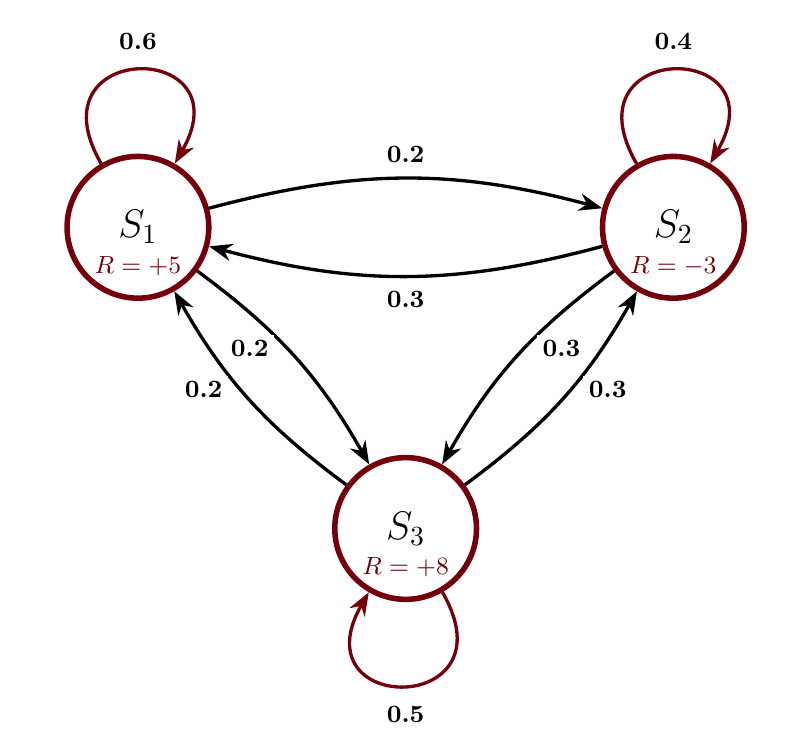
\begin{tikzpicture}[
    >=Stealth,
    scale=0.85,
    every state/.style={
        fill=white,
        draw=USC_Garnet,
        line width=2pt,
        text=black,
        minimum size=1.8cm,
        font=\bfseries\Large
    },
    every edge/.style={
        draw=black,
        line width=1.2pt,
        ->,
        >=Stealth
    },
    prob/.style={
        font=\bfseries\small,
        text=black,
        fill=white,
        inner sep=2pt
    },
    statelabel/.style={
        font=\small\bfseries,
        text=USC_Garnet
    }
]

\node[state] (S1) at (0, 0) {$S_1$};
\node[statelabel, below=1pt of S1.center, yshift=-6pt] {$R=+5$};

\node[state] (S2) at (8, 0) {$S_2$};
\node[statelabel, below=1pt of S2.center, yshift=-6pt] {$R=-3$};

\node[state] (S3) at (4, -4.5) {$S_3$};
\node[statelabel, below=1pt of S3.center, yshift=-6pt] {$R=+8$};

\path (S1) edge[loop above, looseness=5, out=120, in=60, draw=USC_Garnet] node[prob, above=5pt] {0.6} (S1);
\path (S2) edge[loop above, looseness=5, out=120, in=60, draw=USC_Garnet] node[prob, above=5pt] {0.4} (S2);
\path (S3) edge[loop below, looseness=5, out=-60, in=-120, draw=USC_Garnet] node[prob, below=5pt] {0.5} (S3);

\path (S1) edge[bend left=15] node[prob, above=3pt] {0.2} (S2);
\path (S2) edge[bend left=15] node[prob, below=3pt] {0.3} (S1);

\path (S1) edge[bend left=12] node[prob, left=4pt, pos=0.45] {0.2} (S3);
\path (S3) edge[bend left=12] node[prob, left=4pt, pos=0.55] {0.2} (S1);

\path (S2) edge[bend right=12] node[prob, right=4pt, pos=0.45] {0.3} (S3);
\path (S3) edge[bend right=12] node[prob, right=4pt, pos=0.55] {0.3} (S2);

\end{tikzpicture}
\end{document}
